%% ----------------------------------------------------------------
%% Introduction.tex
%% ---------------------------------------------------------------- 




\chapter{Introduction} \label{Chapter:Introduction}
% 区块链技术自发明以来就饱受争议,主要的争议点在于实际应用少,同时虚拟货币需要消耗大量的电力来进行挖矿,而目前全球电力的主要供应来源依然是化石能源,在用有限的化石能源电力时会产生大量排放。各国近年不停的推出严厉的排放政策以期缓解全球变暖以及化石能源枯竭的趋势,在这种背景下,碳排放市场和清洁能源交易逐渐走进人们的眼中,本项目旨在利用区块链技术实现一个无需挖矿的清洁能源电力交易平台,使它具备清洁能源以及其清洁积分交易的功能,使得普通人可以认购清洁能源证书以获取清洁能源积分,并且最后可以将清洁能源积分售卖给需要清洁能源积分的工厂从而形成一个良性的循环,吸引更多普通人参与这种环保行动以达到减少排放且能获得一定的收益的目的。
Blockchain technology has been controversial since its invention, the main point of contention is that there are not many practical applications, while cryptocurrencies need to consume a lot of power for mining \cite{disadvantagecrypto}, and the main source of global power supply is still fossil energy, which generates a lot of emissions when using limited fossil energy power\cite{QI2020115049}. In recent years, countries have been launching severe emission policies to alleviate global warming and the trend of fossil energy depletion, in this context, carbon emission market and clean energy trading gradually come into the eyes of people.

This project aims to use blockchain technology to realize a clean energy power trading platform without mining, so that it has the function of clean power and its clean power points trading. In the system, ordinary people can subscribe to clean energy certificates to obtain clean power points, and finally sell clean power points to factories that need to get emission rights by clean power points. In this way, people contribute to energy saving and emission reduction through clean power trading, while gaining a little profit, forming a virtuous circle of environmental action and promoting the popularity of clean power.

\section{Climate Problem}
As climate and environmental problems are becoming more and more serious, in order to protect the home that human beings depend on, countries have proposed their own schedule of carbon neutrality and carbon peaking in their respective government work reports, and the Japanese government proposed to achieve carbon neutrality by 2050 in October 2020\cite{japanesereport}. The Chinese government has also set a specific time frame for carbon peaking and carbon neutrality in the government work report \cite{chinareport}. According to Zhang \cite{Zhang2020}, the measure of carbon emissions trading for manufacturing companies has been effective in reducing carbon emissions in China for many years, with car companies producing low-emission or no-emission products, such as Tesla and BYD, making huge profits from the sale of carbon emission targets, and car companies producing high-emission products, such as Volkswagen and Geely, actively developing low-emission products and promoting technological progress. Thus,a multi-win situation has been achieved by emission market, however, complete carbon neutrality is a universal goal that requires the participation of everyone, so it is necessary to consider how to allow ordinary citizens to participate in the carbon emissions trading system. The production of electricity accounts for a large proportion of greenhouse gas emissions \cite{Zhu2020}, and electricity is something that everyone touches every day, and as fossil energy sources shrink and become more expensive \cite{Li2021}, clean electricity is gaining attention and is gradually being grid-connected and used on a large scale \cite{Sifat2019}. Therefore, clean power trading is a field in which everyone can participate.

\section{Power Internet}
Based on the concept of Internet Plus \cite{internetplus2016}, China has developed a well-developed power trading system in recent years \cite{energyinternet2015}, which refers to the use of Internet thinking and technology to transform the traditional power industry in order to achieve the deep integration of the Internet with power production, transmission, storage, consumption and power markets \cite{defenergyinternet}, and to create an power ecosystem with equal participation, common construction and governance, and collaborative operation. Among the new generation of information and communication technologies, blockchain technology, as a new distributed infrastructure and bookkeeping technology, can provide a trust basis for multi-party collaboration in the power Internet with its clever technical design and data governance \cite{Bao2020}.

\section{Blockchain Application}
The technical characteristics of blockchain have some similarity with the concept of power Internet, and both embody the ideas of decentralization and autonomous synergy, with the trend of intelligence and contractualization, and both can promote the establishment of market-based platforms \cite{Nofer2017}. Therefore, in recent years, there have been more and more theoretical and practical studies focusing on the application of blockchain technology in the power Internet. The literature \cite{summaryblockchian2019} summarized the typical application scenarios of blockchain in the fields of power supply, transmission, distribution, consumption and trading, and pointed out that blockchain would be the first to be applied in the field of power trading. The literature \cite{blockchainapplication2021} summarized the applications of blockchain technology in the fields of distributed power trading, data management and information security, carbon emission rights certification and green certificate trading, and concluded that scenarios such as distributed power trading are the most priority application areas for development and promotion. The literature \cite{Thu2020} introduced the current engineering status of blockchain+power applications at home and abroad, and pointed out that blockchain has unique advantages when used to solve the problems of renewable power consumption, distributed power trading, and lack of trust among multi-interest entities.



% You probably found all the files from \cite{Gunn:2001:pdflatex}.
% \tref{Table:tabex} illustrates the results of my work.
% \begin{table}[!htb]
%   \centering
%   \begin{tabular}{cc}
%   \toprule
%   \textbf{Training Error} & \textbf{Testing Error}\\
%   \midrule
%   0 & $\infty$\\
%   \bottomrule
%   \end{tabular}
%   \caption{The Results}
%   \label{Table:tabex}
% \end{table}

% \fref{Figure:figex} shows why this is the case.
% \begin{figure}[!htb]
%   \centering
%   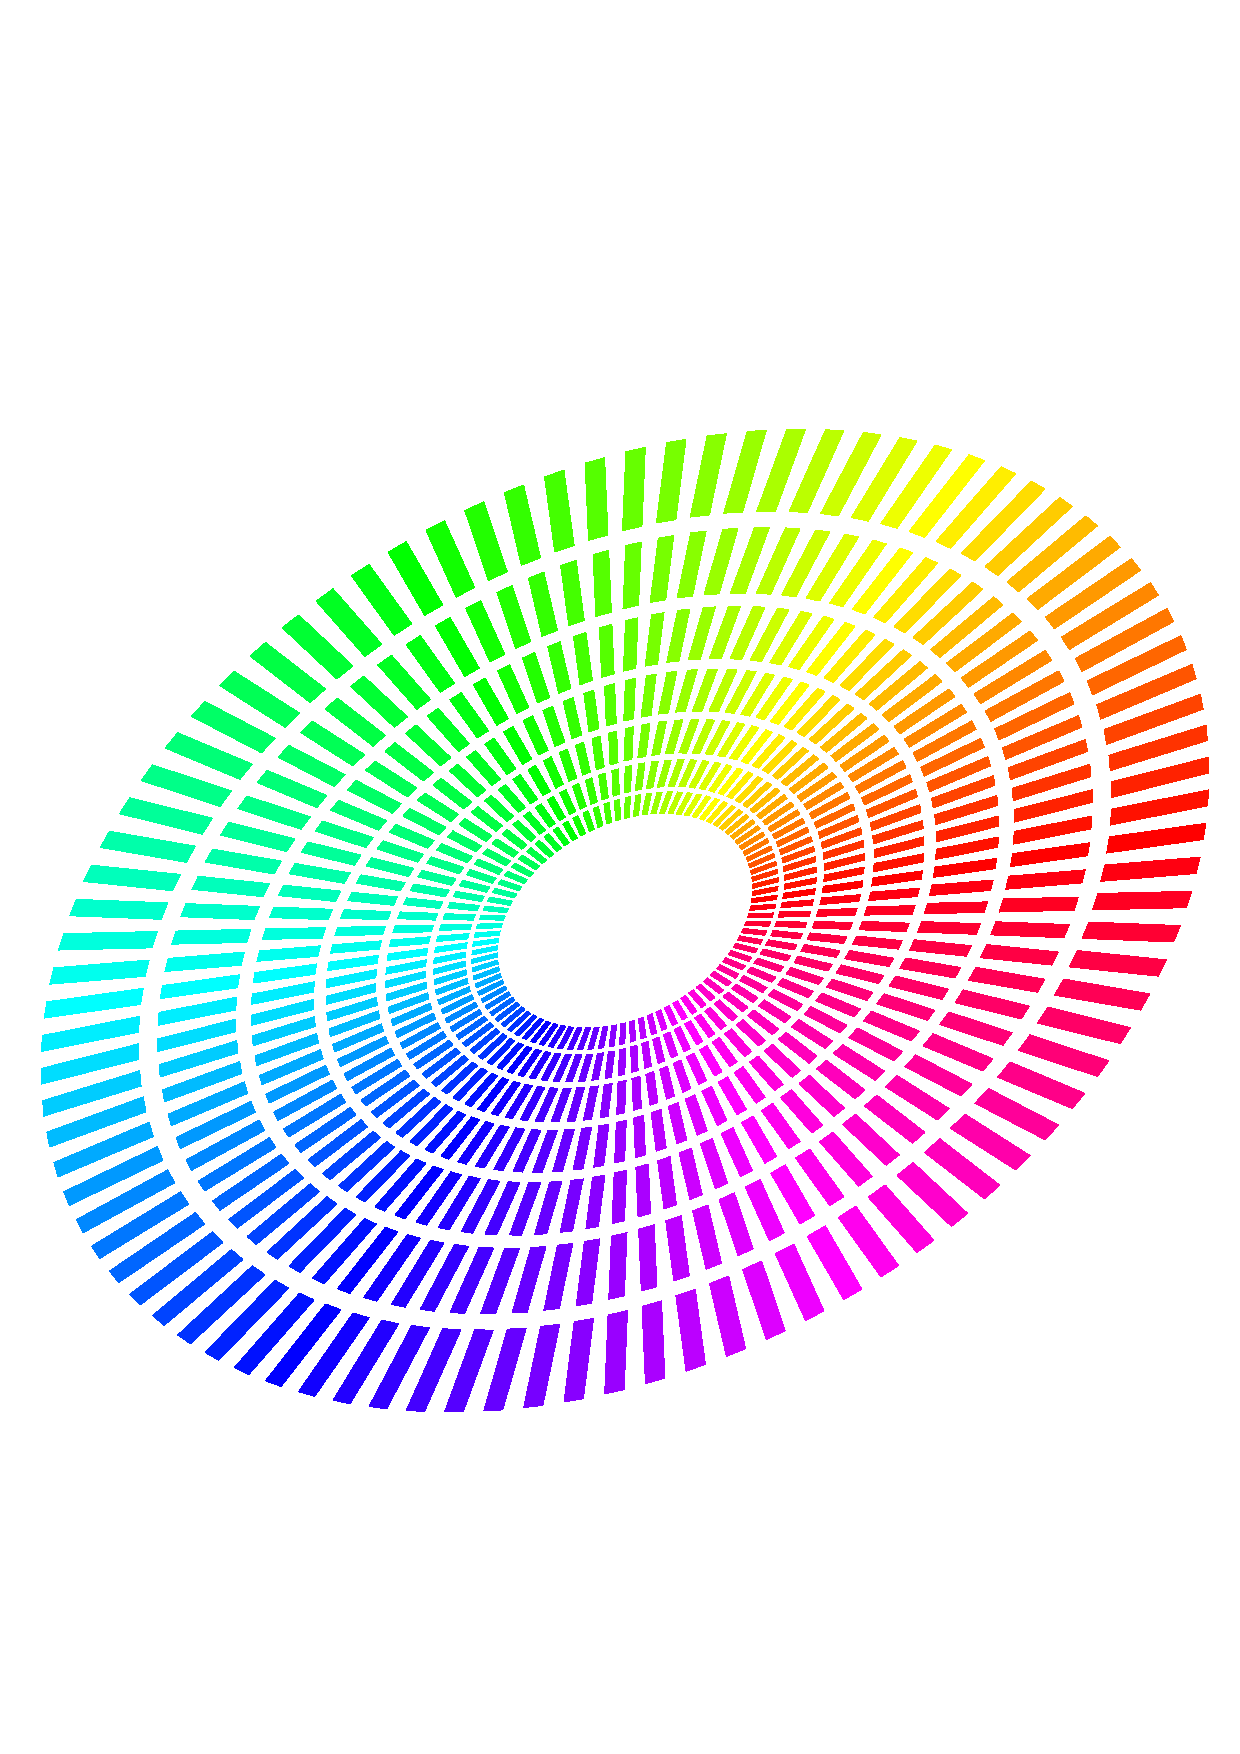
\includegraphics[width=8cm]{figure}
%   \caption{A colourful picture.}
%   \label{Figure:figex}
% \end{figure}

% This page shows you a subfigure example in \fref{Figure:figsubex}.
% \begin{figure}[!htb]
%   \centering
%   \subfigure[The left caption]{
%     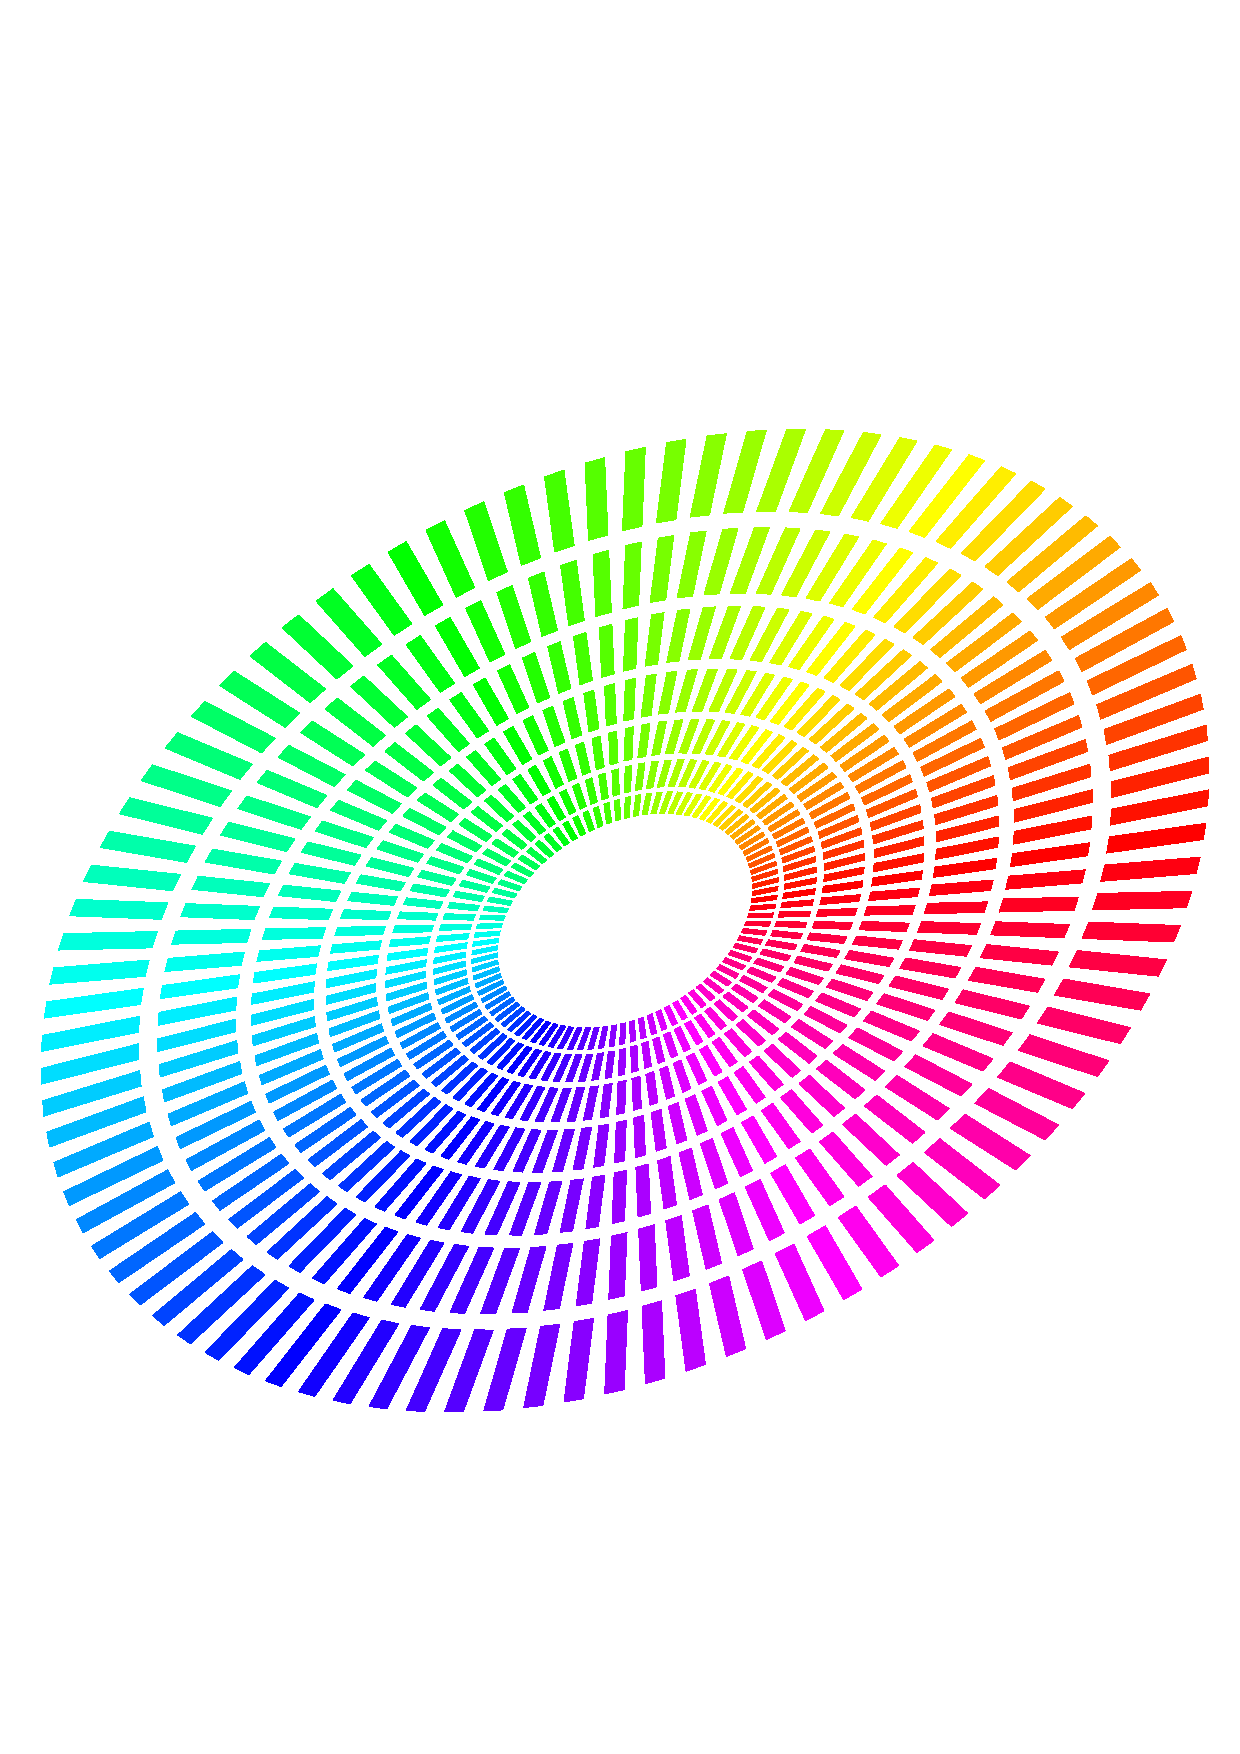
\includegraphics[width=4.2cm]{figure}
%     \label{Figure:figsubex:left}
%   }
%   \subfigure[The right caption]{
%     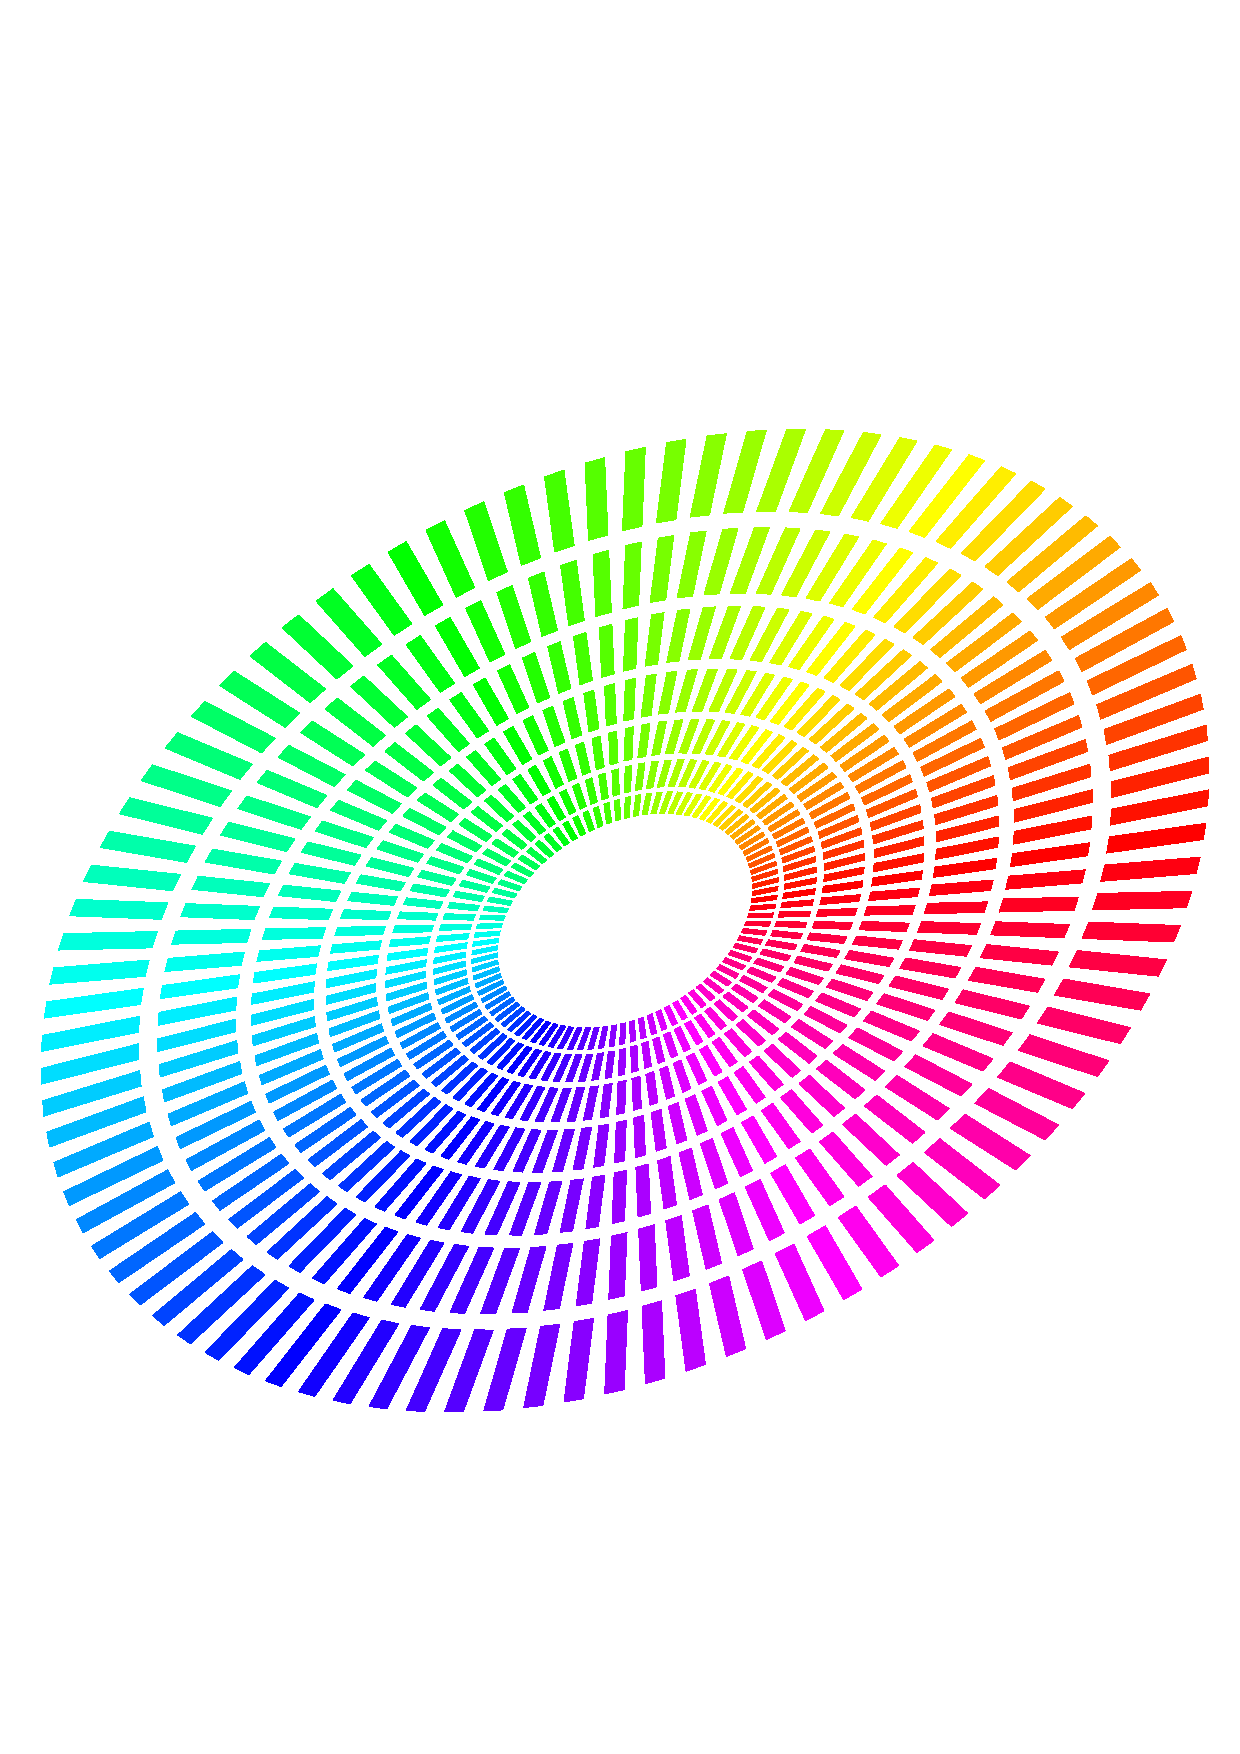
\includegraphics[width=4.2cm]{figure}
%     \label{Figure:figsubex:right}
%   }
%   \caption{A doubly colourful picture.}
%   \label{Figure:figsubex}
% \end{figure}
